%--------------------------------------------------------
%--------------------------------------------------------
%\section{The spin-0 description of CMB polarization} \label{sec:pol-intro}
%--------------------------------------------------------
\section{Polarization primer}\label{sec:pol-primer}
The CMB polarization is measured in terms of Stokes Q and U parameters. The Stokes Q is defined as the linear polarization measured along local cartesian axes ($+$ along the x-axis and $-$ along the y-axis) while Stokes U is defined as the linear polarization measured along the cartesian axes rotated by $45^{\circ}$ ($+$ along x-axis and $-$ along the y-axis in the counter-clockwise rotated system). Clearly the definitions of Stokes parameters depend on the choice of the coordinate system and it can be shown that the measurement made in two different coordinate systems rotated by an angle $\phi$ are related by the following equation,
%
\beq \label{eq:qu-rot}
\fqu' = \begin{bmatrix} \cos{2 \psi} &  \sin{2 \psi} \\ -\sin{2\psi} & \cos{2 \psi} \end{bmatrix} \fqu \,,
\eeq
%
which one can simply checked by verifying that $Q' \rightarrow U$ and $U' \rightarrow -Q$ when the coordinate systems are rotated by $45^\circ$ in the counter-clockwise sense. 

Following the notation of \cite{Zaldarriaga1997}, fields which transform as,
%
\beq
{}_{s}f' = e^{-is\psi} {}_{s}f \,,
\eeq
%
under right handed rotations of the local coordinate system are termed spin-s fields. The Stokes parameters can be combined to define the complex fields,
%
\beq \label{eq:spin-pol}
_{\pm 2}\bar{X}(\hat{n}) = Q(\hat{n}) \pm i U (\hat{n}) \,, %\nonumber \\ &=& \sum_{\ell m}  {_{\pm 2}} \tilde{X}_{\ell m}  \, {_{\pm 2}}Y_{\ell m} (\hat{n}) \,.
\eeq
%
which under rotation of the local tangent plane coordinate system by an angle $\psi$ at any point on the sphere transform as: $_{\pm 2}X' = e^{\mp i2\psi} {_{\pm 2}X}$, which follows directly from \eq{eq:qu-rot}. Therefore the quantities $_{\pm2}X$ are spin${\pm2}$ fields respectively.

The Stokes parameters being coordinate dependent quantities it is inconvenient to work with them. It is possible to define spin raising ($\eth$) operator on the sphere which when operated on a field of spin-s $_{s}f$ results in a fields with spin-$(s+1)$: $(\eth _{s}f)' = e^{-i(s+1)\psi}(\eth _{s}f)$ and similarly one can define a spin lowering $(\bar{\eth})$ operators such that $(\bar{\eth} _{s}f)' = e^{-i(s-1)\psi}(\bar{\eth} _{s}f)$\cite{goldberg67}. One can now construct a complex spin-0 scalar by applying the spin raising and lowering operators on the spin-2 fields ${_{\pm 2}X}$ as follows,
%
\begin{subequations}\label{eq:ebdef}
\beqry
\mathcal{E}(\hat{n}) + i \mathcal{B}(\hat{n}) &=& -\bar{\eth}^2 _{+ 2}\bar{X}(\hat{n}) \,,\\
\mathcal{E}(\hat{n}) - i \mathcal{B}(\hat{n}) &=& -{\eth}^2 _{-2}\bar{X}(\hat{n}) \,,
\eeqry
\end{subequations}
%
which by the virtue of being scalars are independent of coordinate definitions. %The real part of this complex spin-0 scalar field corresponds to the E-mode while the imaginary part to the B-modes \cite{Kamionkowski1997}. 

The complex field $_{\pm 2}X$ defined on the sphere can be decomposed in spin spherical harmonic functions: ${}_{\pm 2}X(\hat{n}) = \sum_{\ell m} {}_{\pm 2} X_{\ell m} {}_{\pm 2}Y_{\ell m}(\hat{n})$. On applying the spin raising and lowering operators on the spin spherical harmonic functions leads to the following identities\cite{goldberg67},
%
\begin{subequations}\label{eq:spinopylm} 
\beqry
\eth _s Y_{lm}(\hat{n}) &=& \sqrt{(\ell-s)(\ell+s+1)} _{s+1} Y_{lm}(\hat{n}) \,, \\
\bar{\eth} _s Y_{lm}(\hat{n}) &=& -\sqrt{(\ell+s)(\ell-s+1)} _{s-1} Y_{lm}(\hat{n}) \,, 
\eeqry
\end{subequations}
%
where $_s Y_{lm}(\hat{n}) $ denote the spin-s spherical harmonics.

Using \eq{eq:ebdef}, the spin spherical harmonic decomposition of ${}_{\pm2}X$ and the identities given in \eq{eq:spinopylm} it can be shown that the scalar fields $\mathcal{E}/\mathcal{B}$ are given by the following equations,
%
\beq \label{eq:pseudo}
\mathcal{E}(\hat{n}) = \sum_{\ell m} a^{E}_{\ell m} \sqrt{\frac{(\ell+2)!}{(\ell-2)!}} Y_{\ell m} (\hat{n}) ~\,;~ \mathcal{B}(\hat{n})  =\sum_{\ell m} a^{B}_{\ell m} \sqrt{\frac{(\ell+2)!}{(\ell-2)!}} Y_{\ell m} (\hat{n}) \,,
\eeq
%
where the harmonic coefficients $a^{E}_{\ell m}$  \& $a^{B}_{\ell m}$ are related to the harmonic coefficients of the spin-2 polarization field via the following equations,
%
\beq\label{eq:x2eb}
a^{E}_{\ell m} = -\frac{1}{2} \Big[ {}_{+2}\tilde{X}_{\ell m} + {}_{-2}\tilde{X}_{\ell m} \Big] ~\,;~a^{B}_{\ell m} = -\frac{1}{2i} \Big[ {}_{+2}\tilde{X}_{\ell m} - {}_{-2}\tilde{X}_{\ell m} \Big] \,.
\eeq
%
In the remainder of this article, we will work with the scalar $E$ and pseudo scalar $B$ fields as defined by the following equations, 
%
\beq \label{eq:realeb}
E(\hat{n}) = \sum_{\ell m} a^{E}_{\ell m} Y_{\ell m} (\hat{n}) ~\,;~ B(\hat{n})  =\sum_{\ell m} a^{B}_{\ell m} Y_{\ell m} (\hat{n}) \,.
\eeq
%
Note that these $E/B$ fields are merely filtered versions of $\mathcal{E}/\mathcal{B}$ as their spherical harmonic coefficients of expansion are related by the factor $\sqrt{\frac{(\ell+2)!}{(\ell-2)!}}$. %We make this choice since the CMB spectra are more closely related to the fields E \& B.
%--------------------------------------------------------
%--------------------------------------------------------
\subsection{Matrix notation} \label{sec:mat_pol_intro}
In this section we cast the relations introduced in Sec.~\ref{sec:pol-primer} in matrix notation\footnote{While we work with the matrix and vector sizes given in terms of some pixelization parameter $\rm N_{\rm pix}$, all the relations are equally valid in the continuum limit attained by allowing $\rm N_{\rm pix}\rightarrow \infty$}. This representation will make transparent the derivation of the real space operators we discuss in the following sections. We adopt a convention in which real space quantities are denoted by bar-ed variable while those in harmonic space are denoted by tilde-ed variables.

We begin by introducing the matrices encoding the spin spherical harmonic basis vectors,
%
\beq
{}_{|s|}\mathcal{Y}= \bmat _{+s}Y & 0 \\ 0 & _{-s}Y \emat _{2 \rm N_{\rm pix} \times 2 \rm N_{\rm alms}} \,,
\eeq
%
where $s$ denotes the spin of the basis functions. For this work we will be working with cases $s \in [0,2]$. In this notation, each column can be mapped to a specific harmonic basis function marked by the pair of indices: $(\ell,m)$ and each row maps to a specific position on the sphere. Note that this matrix is in general not a square matrix. The number of rows is determined by the scheme used to discretely represent the sphere and the number of columns is set by the number of basis functions of interest (often determined by the band limit).

We now define the different polarization data vectors and their representation in real and harmonic space as follows,
%
\beqrys
\bar{S} &=& \bmat E \\ B  \emat_{2 \rm N_{\rm pix} \times 1} ~~~~;~~ \bar{X} = \bmat _{+2}X \\ _{-2}X \emat_{2 \rm N_{\rm pix} \times 1} ~~;~~\bar{P} =\fqu_{\tiny {2 \rm N_{\rm pix} \times 1}} \,, \\
\tilde{S} &=& \bmat a^{E} \\ a^{B} \emat _{2 \rm N_{\rm alms} \times 1}  ~~; ~~ \tilde{X} = \bmat _{+2} \tilde{X} \\ _{-2} \tilde{X} \emat_{2 \rm N_{\rm alms} \times 1} \,.
\eeqrys
%
The different symbols have the same meaning as that discussed in \sec{sec:pol-primer}, except that the subscript $_{\ell m}$ for the spherical harmonic coefficients of expansion is suppressed in favor of cleaner notation.

Next we define the operators which govern the transformations between different representations of the polarization field as follows,
%
\beqrys
\bar T &=& \qutox_{2 \rm N_{\rm pix} \times 2 \rm N_{\rm pix}} ~~;~~ \bar T^{-1} = \frac{1}{2} \bar T^{\dagger} \,, \\
\tilde T &=& -\qutox_{2 \rm N_{\rm alms} \times 2 \rm N_{\rm alms}} ~~;~~ \tilde T^{-1} = \frac{1}{2} \tilde T^{\dagger} \,,
\eeqrys
%
where we have chosen the sign conventions so as to match those used in Healpix.
Using the data vectors and the matrix operators defined above we can now express, in compact notation, the forward and inverse relations between different representations of the polarization data vectors as follows,
%
\begin{subequations} \label{eq:pol_data_relns}
\beqry 
\bar{X} &=& \bar T * \bar{P} ~~;~~\bar{P} = \frac{1}{2} \bar T^{\dagger} * \bar{X} \,, \\
\bar X &=&  {{}_2\mathcal{Y}} * \tilde X  ~~;~~ \tilde X ={{}_2\mathcal{Y}}^{\dagger} * \bar X  \,, \\
\tilde{X} &=& \tilde T * \tilde{S} ~~;~~ \tilde{S} = \frac{1}{2}\tilde T^{\dagger} * \tilde{X} \,.\\ 
\bar S &=&  {{}_0\mathcal{Y}} * \tilde S ~~;~~  \tilde S =  {{}_0\mathcal{Y}}^{\dagger} * \bar S \,.
%\tilde X &=&  {{}_2\mathcal{Y}}^{\dagger} * \bar X ~~;~~ \tilde{X} = \tilde T * \tilde{S} \,, \\
%\bar{S} &=& {{}_0\mathcal{Y}}*\tilde S ~~;~~ \tilde{S} = \frac{1}{2}\tilde T^{\dagger} * \tilde{X} \,.\\
%\bar{X} &=& \bar T * \bar{P} ~~;~~ \tilde{X} = \tilde T * \tilde{S} \,, \\
%\bar{P} &=& \frac{1}{2} \bar T^{\dagger} * \bar{X} ~~;~~ \tilde{S} = \frac{1}{2}\tilde T^{\dagger} * \tilde{X} \,. \\
\eeqry
\end{subequations}
%
Finally we introduce the harmonic space operators, which project the harmonic space data vector to E or B subspace,
%
\begin{subequations} \label{eq:har_eb_op}
\beqry
\tilde O_E &=& \bmat \mathbb{1} & \mathbb{0} \\ \mathbb{0} & \mathbb{0} \emat _{2 \rm N_{\rm alms} \times 2 \rm N_{\rm alms} }   ~~;~~ \tilde S_E = \tilde O_E* \tilde S \,,\\
\tilde O_B &=& \bmat \mathbb{0} & \mathbb{0} \\ \mathbb{0} & \mathbb{1} \emat _{2 \rm N_{\rm alms} \times 2 \rm N_{\rm alms} } ~~; ~~ \tilde S_B = \tilde O_B *\tilde S \,
\eeqry
\end{subequations}
%
Note that these harmonic space matrices are idempotent, orthogonal to each other and their sum is an identity matrix as can be explicitly seen via the following relations, 
%
\begin{subequations} \label{eq:har_op_prop}
\beqry
\tilde O_E * \tilde O_E&=& \tilde O_E ~~;~~  \tilde O_B * \tilde O_B= \tilde O_B \,,\\
 \tilde O_E * \tilde O_B&=& \mathbb{0} \,, \label{eq:op_eb_ortho}\\ 
 \tilde O_E + \tilde O_B&=& \mathbb{1} \,.
\eeqry
\end{subequations}
%
Note that the above relations for these harmonic space operators are exactly valid.  In the following sections we aim to derive the real space analogues of these harmonic space operators.
%%%%%%%%%%%%%%%%%%%%%%%%%%%%%%%%%%%
\section{Real space operators} \label{sec:real_space_operators}
The vector-matrix notation introduced in  \sec{sec:mat_pol_intro} allows for concise book keeping of all the operations involved in the analysis of CMB polarization. In this section we use this notation to derive the real space operators which translate the Stokes vector \vp{}  to the vector of scalars \vs  and vice versa. This vector-matrix notation also allows us to simply derive real space operators for direct decomposition of the Stokes vector \vp{} in to a vector \vp{ E} that correspond to $E$-modes and another vector \vp{B} that corresponds to the $B$-modes of polarization, such that \vp{} = \vp{E} + \vp{B}, without ever evaluating the $E$ \& $B$ fields or their spherical harmonics. 
All the real space operators we derive are most conveniently expressed as functions of the Euler angles  $\alpha, ~\beta~\&~ \gamma$ on the sphere. Owing to this, we begin with a brief discussion on Euler angles and \revisit{present a visual method to think about them.}
%
\begin{figure}[!hbt]
\centering
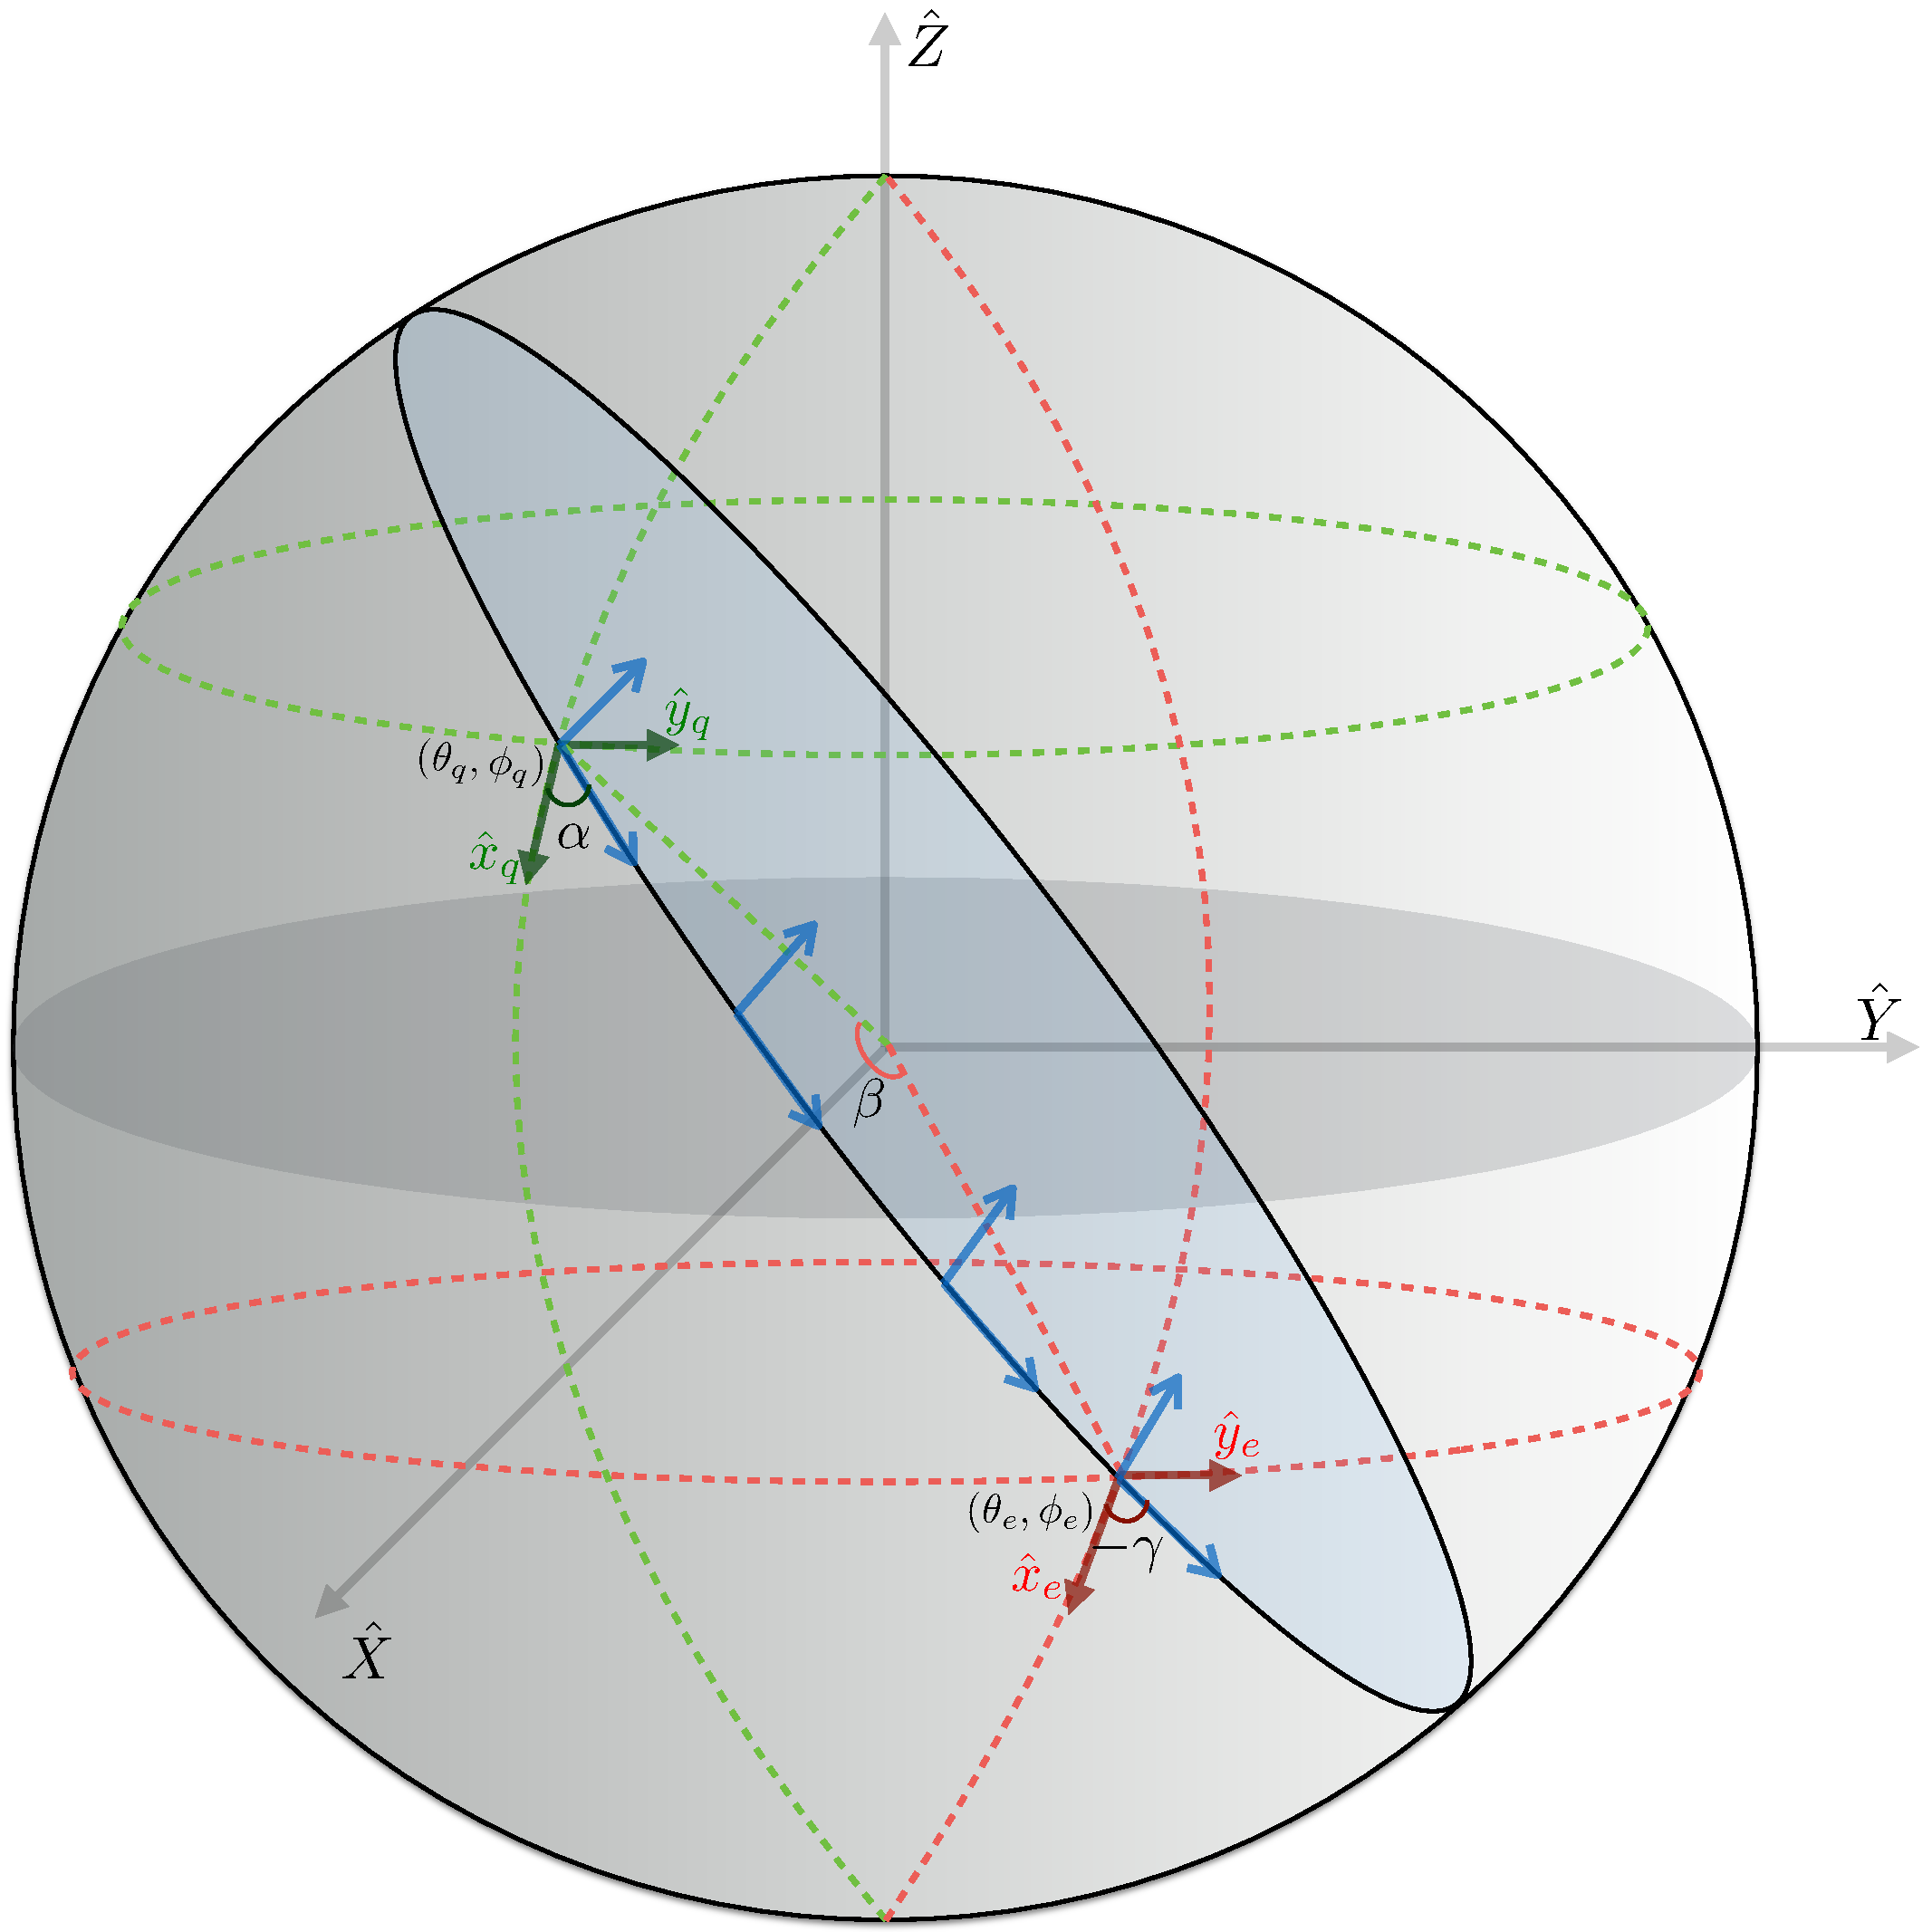
\includegraphics[width=0.5\columnwidth]{euler.pdf}
\caption{This figure depicts the Euler angles in the z-y1-z2 convention. The cartesian coordinates shown in dark green are those that lie in the tangent plane at location $\hat{n}_q = (\theta_q, \phi_q)$ while those shown in dark red are the ones that lie in the tangent plane at location $\hat{n}_e = (\theta_e, \phi_e)$. The blue coordinates at different locations are representative of the parallel transport along the geodesic connection the two locations $\hat{n}_q$ \& $\hat{n}_e$ on the sphere.}
\label{fig:euler_angles}
\end{figure}
%

\textit{Euler angles:}  We define the local cartesian coordinate system at any point on the sphere such that the z-axis points along the radial direction, the x-axis is along the vector tangent to the local longitude pointing south and the y-axis is a vector tangent to the local latitude pointing east as shown in \fig{fig:euler_angles}. The Euler angles $\alpha ,\beta ~\&~ \gamma$ define rotation operations that transforms the local cartesian coordinate system defined at the location $\hat{n}_q \equiv (\theta_q,\phi_q)$ such that it aligns with the local cartesian coordinate system at the location $\hat{n}_e \equiv (\theta_e,\phi_e)$ \cite{varshalovich}. 

For this work, it is convenient to think in the z-y1-z2 convention therefore all future references to Euler angles are in this convention\footnote{The Euler angles in the more standard $z-y-z$ convention are related to those in the $z-y1-z2$ convection by the following rule: $(\alpha,\beta,\gamma)_{z-y-z} =(\gamma,\beta,\alpha)_{z-y1-z2}$ \cite{varshalovich}.}.
In the z-y1-z2 convention, $\alpha$ defines the rotation about the z-axis, $\beta$ defines the rotation about the new y-axis (y1-axis) after the previous rotation and $\gamma$ defines the rotation about the final z-axis (z2-axis) after carrying out the previous two rotations. These angles can be understood as follows: The rotation by $\alpha$ about the original z-axis is such that it aligns the x-axis of the cartesian system at location $\hat{n}_q$ along the great circle in the direction \revisit{of shortest arc length} towards $\hat{n}_e$.  The rotation by $\beta$ about the y2-axis parallel transports the local cartesian coordinate system from location $\hat{n}_q$ to location $\hat{n}_e$, such that the z-axes of the two coordinate systems are parallel to each other. Finally the rotation by angle $\gamma$ about the z2-axis aligns the x \& y axes of the parallel transported system with those of the local cartesian system defined at $\hat{n}_e$. The different Euler angles and the corresponding rotations are schematically represented in \fig{fig:euler_angles}.

The simplest scenario is when one of the coordinates coincides with the north pole $\hat{n}_q=(\theta_q,\phi_q)=(0,0)$ (the local cartesian system at this point being defined with an arbitrary convention set by choosing $\theta_0 \rightarrow 0$ while moving along the longitude $\phi_0=0$), in which case it is easy to see that rotations by Euler angles: $(\alpha,\beta,\gamma) =(\phi_e,\theta_e,0)$ will align the cartesian system at $\hat{n}_q$ with that defined at position $\hat{n}_e$. 
%--------------------------------------------------------

%--------------------------------------------------------
\subsection{A heuristic argument for constructing  $E/B$ modes from Stokes parameters $Q/U$ on the sphere} \label{sec:qu2eb_heuristic}
The primary aim here is to make intuitive the construction of the spin-0 $E/B$ modes of polarization from the Stokes parameters. We present heuristic arguments which allows us to derive the important features of the real space kernels\footnote{These heuristic arguments were developed in hindsight but are very instructive.}. 

If one rotates the cartesian coordinates in the tangent plane at location $\hat{n}_q$ by an angle $\phi$ about the local $\hat{z}_q$ axis, the Stokes charge in the new coordinate system is related to the Stokes charge in the original coordinate system as: ${}_{+2}X'(\hat{n}_q) \xrightarrow{\mathcal{R}_{\hat{z}_q}(\phi)} {}_{+2}X(\hat{n}_q) e^{-i2\phi} $. Similarly if the local planar axes are rotated by an angle $\phi$ then the Euler angle $\alpha_{qe}$ (recall that this Euler angle aligns the x-axis at $\hat{n}_q$ in the direction of the shortest path along the geodesic to the location $\hat{n}_e$) for the new coordinate system is given by: $\alpha'_{qe} \rightarrow \alpha_{qe} - \phi$ and therefore one can see that: $e^{-i2\alpha'_{qe}} \xrightarrow{\mathcal{R}_{\hat{z}_q}(\phi)} e^{-i2\alpha_{qe}} e^{i2\phi}$. The Euler angles $|\beta_{qe}|$ which measure the angular distance between pixels remains unaltered under this local rotation operation.  Given these transformation properties note that: ${}_{+2}X'(\hat{n}_q)e^{-i2\alpha'_{qe}} \xrightarrow{\mathcal{R}_{\hat{z}_q}(\phi)} {}_{+2}X(\hat{n}_q) e^{-i2\alpha_{qe}}$ is invariant under rotations  $\mathcal{R}_{\hat{z}_q}(\phi)$ and hence by definition must form a spin-0 field.  Now note that the real part of the function are constructed by product of functions $(Q\cos{2\alpha}, U\sin{2 \alpha})$ having the same parity and hence the real part must have even parity while the imaginary part of the function are constructed by multiplying functions $(Q\sin{2 \alpha}, U\cos{2\alpha})$ of opposite parity and hence must have an odd parity. Therefore we can make the association: $E'+iB' \propto {}_{+2}X(\hat{n}_q) e^{-i2\alpha_{qe}}$

Now note that when the two locations coincide $\hat{n}_q = \hat{n}_e$ then  $\alpha_{qe}=0,2\pi,4\pi,\cdots$ implying $E + iB \propto Q+iU$, which is a fallacy as we know that $Q+iU$ does not transform as a spin-0 field under local rotations. One runs into a similar fallacy when the two locations are diametrically opposite.  Therefore to have a consistent definition of a spin-0 field constructed from a spin-2 field we require the kernel to have the form: $E'+iB' = {}_{+2}X(\hat{n}_q) f(\beta_{qe})  e^{-i2\alpha_{qe}}$, where the function $f(\beta_{qe})$ is such that it vanishes when the two locations are coincident$(\beta_{qe}=0)$ or diametrically opposite$(\beta_{qe}=\pi)$. Hence the $E/B$ fields are necessarily non-local. Note that this construction can be generalized to transform fields of arbitrary spin to a field of any other spin, one obvious case being constructing the Stokes field given the $E/B$ maps (i.e. deriving spin-2 fields from spin-0 fields.)

The azimuthal part which depends only on the Euler angle $\alpha_{qe}$, has no multipole $\ell$ dependence and is the crucial operation which translates between the different spin representation of CMB polarization. Only the radial part of the kernel $f(\beta_{qe})$ depends only on the angular separation $|\beta_{qe}|$ between different locations on the sphere and hence must completely incorporate the multipole $\ell$ dependence of the kernel. These heuristic arguments cannot take us any further and we now shift to presenting a mathematically rigorous derivation of the real space operators in the following sections. 
%--------------------------------------------------------


%--------------------------------------------------------
\subsection{Evaluating scalar fields $E$ \& $B$ from Stokes parameters $Q$ \& $U$}\label{sec:qu2eb}
In \sec{sec:pol-primer} we described the conventional procedure of computing the scalar fields E \& B from the Stokes parameters Q \& U. 
%To reiterate, this process involved taking the spin harmonic transform of the complex spin-2 fields ${}_{\pm2} \bar X$, forming specific linear combinations of the resultant coefficients of expansion ${}_{\pm 2} \tilde X_{\ell m}$ and evaluating the forward spin-0 transform to derive the scalar E \& B fields. 
In this section we derive the real space convolution kernels on the sphere which can be used to directly evaluate the scalar fields $E$ \& $B$ on the sphere.  We use the vector-matrix notation introduced in \sec{sec:mat_pol_intro} to write down an operator equation relating the real space vector of scalars \vs to the Stokes polarization vector \vp{},
%
\beqrys
\bar{S} &=& {{}_0\mathcal{Y}} *\tilde T^{-1}* {{}_2\mathcal{Y}^{\dagger}} *\bar T *\bar{P} = \frac{1}{2} {{}_0\mathcal{Y}} *\tilde T^{\dagger} *{{}_2\mathcal{Y}^{\dagger}} *\bar T *\bar{P}   \,, \\
&=&  \bar O *\bar{P} \,. \label{eq:qu2eb_op}
\eeqrys
%
The explicit form of the real space operator $\bar O$ can be derived by contracting over all the matrix operators. This procedure is explicitly worked out in the following set of equations,
%
\beqrys
\bar{O} &=& \frac{1}{2} {{}_0\mathcal{Y}} *\tilde T^{\dagger} *{{}_2\mathcal{Y}^{\dagger}} *\bar T \,, \\
&=& -0.5 \yzmat{e} \qutoxd \ymatc{q} \qutox   \,, \\
&=& -0.5 \begin{bmatrix} \sum ({}_{0}Y_e ~{}_{2}Y^{T*}_q  +  {}_{0}Y_e~ {}_{-2}Y^{T*}_q) & {\rm i}  \sum ({}_{0}Y_e ~ {}_{2}Y^{T*}_q - {}_{0}Y_e ~{}_{-2}Y^{T*}_q)  \\  - {\rm i} \sum  ({}_{0}Y_e ~ {}_{2}Y^{T*}_q - {}_{0}Y_e~ {}_{-2}Y^{T*}_q) & \sum ({}_{0}Y_e~ {}_{2}Y^{T*}_q + {}_{0}Y_e ~{}_{-2}Y^{T*}_q)  \end{bmatrix} \,, \label{eq:qu2eb_ker_1}
\eeqrys
%
where the symbol ${}_{0}Y_e$ is used to denote the sub-matrix ${}_{0}Y_{\hat{n}_e \times \ell m} \equiv {}_{0}Y_{\ell m}(\hat{n}_e)$, the symbol ${}_{\pm 2}Y^{T*}_q$ is used to denote the transposed conjugated matrix ${}_{\pm 2}Y^*_{\ell m \times \hat{n}_q} \equiv {}_{\pm 2}Y^*_{\ell m}(\hat{n}_q)$ and the summation is over the multipole indices $\ell,m$. Note that here we purposefully introduce the notation of the index ``e'' to denote the location where the scalar fields are being evaluated and the index ``q'' to denote the location from which  the Stokes parameters are being accessed. Using the conjugation properties of the spin spherical harmonic functions it can be shown that the following identity holds true,
%
\beq
 \left [\sum_{\ell m} {}_{0}Y_{\ell m}(\hat{n}_e){}_{+2}Y^*_{\ell m}(\hat{n}_q)\right]^* = \sum_{\ell m} {}_{0}Y_{\ell m}(\hat{n}_e){}_{-2}Y^*_{\ell m}(\hat{n}_q) \,,
 \eeq
 %
where the terms on either side of the equation are those that appear in \eq{eq:qu2eb_ker_1}. Note that the operator $\bar{O}$ is real as one expects, since each sub-matrix in \eq{eq:qu2eb_ker_1} is formed by summing a complex number and its conjugate. 

\noindent \eq{eq:qu2eb_ker_1} already presents a real space operator, but it is not in a form which can be practically implemented. To arrive at a real space operator which is practially usable, we use the fact that the $m$ sum over the product of two spin spherical harmonic functions can be expressed as a function of the Euler angles\cite{varshalovich},
%
\beq \label{eq:sum_spin_shf}
 \sum_{m}{{}_{s_1}Y}^*_{\ell m}(\hat{n}_i)\,{{}_{s_2}Y}_{\ell m}(\hat{n}_j) = \sqrt{\frac{2\ell+1}{4 \pi}} {{}_{s_2}}Y_{\ell \,-s_1}(\beta_{ij},\alpha_{ij}) e^{- i s_2 \gamma_{ij}} \,,
\eeq
%
where $\alpha_{ij}, ~\beta_{ij} ~\&~ \gamma_{ij}$ denote the Euler angles that specifically transform $(i \rightarrow j)$: the coordinate system at $\hat{n}_i$ so as to allign the coordinate system at $\hat{n}_j$\footnote{The sense of the rotation become more obvious when this equation is written in terms of the Wigner-D functions.}. The different parts of the real space operator $\bar{O}$  are completely specified by the complex function,
%
\begin{subequations}\label{eq:qu2eb_gen_kernel}
\beqry
\mathcal{M}( \hat{n}_e, \hat{n}_q)  &=& \mathcal{M}_{r} + i \mathcal{M}_{i}  \,,\nonumber \\ 
&=&\sum_{\ell m} {{_0}Y}_{\ell m}(\hat n_e) \, {{_{-2}}Y}^*_{\ell m}(\hat n_q) = \sum_{\ell} \sqrt{\frac{2\ell+1}{ 4 \pi}}{{_0Y}_{\ell 2}}(\beta_{qe},\alpha_{qe})\,,\\
&=&  \Big [ \cos(2 \alpha_{qe}) + i \sin(2 \alpha_{qe} ) \Big]   \sum_{\ell=\ell_{\rm min}}^{\ell_{\rm max}} {\frac{2\ell+1}{ 4 \pi}} \sqrt{\frac{(\ell-2)!}{(\ell+2)!}}P_{\ell 2} (\cos\beta_{qe}) \,, \label{eq:rad_ker_queb} \\
&=&  \Big [ \cos(2 \alpha_{qe}) + i \sin(2 \alpha_{qe} ) \Big] {{}_{\mm}f}(\beta_{qe},\ell_{\rm min},\ell_{\rm max}) \,, 
\eeqry
\end{subequations}
%
where we have used the identity in \eq{eq:sum_spin_shf} to simplify the product of the spherical harmonic functions. Note that the function on the right depends only on two out of the three Euler angles. Employing \eq{eq:qu2eb_gen_kernel} to simplify the product of spherical harmonic functions in \eq{eq:qu2eb_ker_1}, the real space operator $\bar{O}$ can now be cast in this more useful form,
%
\beq\label{eq:op_qu2eb_rad}
\bar O =-\bmat  \mathcal{M}_{r} & \mathcal{M}_{i} \\  -\mathcal{M}_{i}  & \mathcal{M}_{r} \emat_{2 N_{\rm pix} \times 2 N_{pix}} = -{{}_{\mm}f}(\beta_{qe},\ell_{\rm min},\ell_{\rm max})\bmat \cos(2 \alpha_{qe}) & \sin(2\alpha_{qe})\\  -\sin(2 \alpha_{qe})  & \cos(2 \alpha_{qe}) \emat \,,
\eeq
%
where, we reiterate, $\alpha_{qe}, ~\beta_{qe} ~\&~ \gamma_{qe}$ denote the Euler angles which rotate the local cartesian system at $\hat{n}_q$ (location where Stokes parameters are accessed) to the cartesian system at  $\hat{n}_e$ (location where the scalar fields are evaluated): $\hat{n}_q \xrightarrow{\mathcal{R}(\alpha_{qe},\beta_{qe},\gamma_{qe})} \hat{n}_e$. 

\textit{Radiating kernel:} Using \eq{eq:op_qu2eb_rad} in \eq{eq:qu2eb_op} one can see that the $E$/$B$ contribution of the Stokes parameters at some location $\hat{n}_q$ is given by the following expression,
%
\beq  \label{eq:qu2eb_radiation_explicit}
\bar{S}_q = \bmat E_e \\ B_e  \emat_{q} =- {{}_{\mm}f}(\beta_{qe},\ell_{\rm min},\ell_{\rm max})\bmat \cos(2 \alpha_{q e}) & \sin(2\alpha_{q e})\\  -\sin(2 \alpha_{q e})  & \cos(2 \alpha_{q e}) \emat  \bmat Q_{q} \\ U_{q}  \emat \Delta \Omega \,.
\eeq
%
The total map of E \& B modes can be simply evaluated by summing over the contribution from the Stokes parameters at each location $\hat{n}_q$ : $\bar{S} = \sum_{q=1}^{N_{\rm pix}} \bar{S}_q$. This operation can be cast in a concise form as follows,
%
\begin{subequations} \label{eq:qu2eb_radiation_concise}
\beqry 
\left[E + iB\right](\hat{n}_e) &=& -\Delta \Omega  \sum_{q=1}^{N_{\rm pix}} \Big[ {}_{+2}X(\hat{n}_{q}) e^{-i2\alpha_{q e}} \Big]  {{}_{\mm}f}(\beta_{q e}) \,, \\
&=&    \sum_{q=1}^{N_{\rm pix}} \Bigg\lbrace {}_{+2}X(\hat{n}_{q}) \cdot \left[ - \Delta \Omega \sum_{\ell=\ell_{\rm min}}^{\ell_{\rm max}} \sqrt{\frac{2 \ell+1}{4 \pi}}Y^*_{\ell 2}(\beta_{qe},\alpha_{qe}) \right] \Bigg\rbrace \,, \\
&=& \sum_{q=1}^{N_{\rm pix}} {}_{+2}X(\hat{n}_{q}) \cdot  \mathcal{M}_{G}[\hat{n}_q] \,,
\eeqry
\end{subequations}
%
where ``$\cdot$'' denotes a simple scalar multiplication. $\mathcal{M}_{G}$ is merely the conjugated function $\mm^*$ when expressed as a function of the Euler angle $\alpha_{qe}$ and it can be thought of as the Green's function of the operator, since $[E +iB] = \mathcal{M}_{G}$ is the spin-0 scalar field generated from the Stokes charge $[Q+iU] = [\delta(\hat{n}-\hat{n}_q) + i 0]$. 

We denote the kernel expressed in terms of the Euler angle $\alpha$ as the radiating kernel, since it allows us to evaluate the $E/B$ field contribution across the sphere due to a single Stoke (charge) parameter at a fixed location on the sphere. The total $E/B$ maps can then be thought of as just superposed radiation emerging from Stokes charges across the sphere. In this formulation, one is effectively in the frame of the Stokes charge ${}_{\pm2}X$ and evaluating its contribution to the complex spin-0 scalar field across the sphere. 
%
\begin{figure}[!t]
\centering
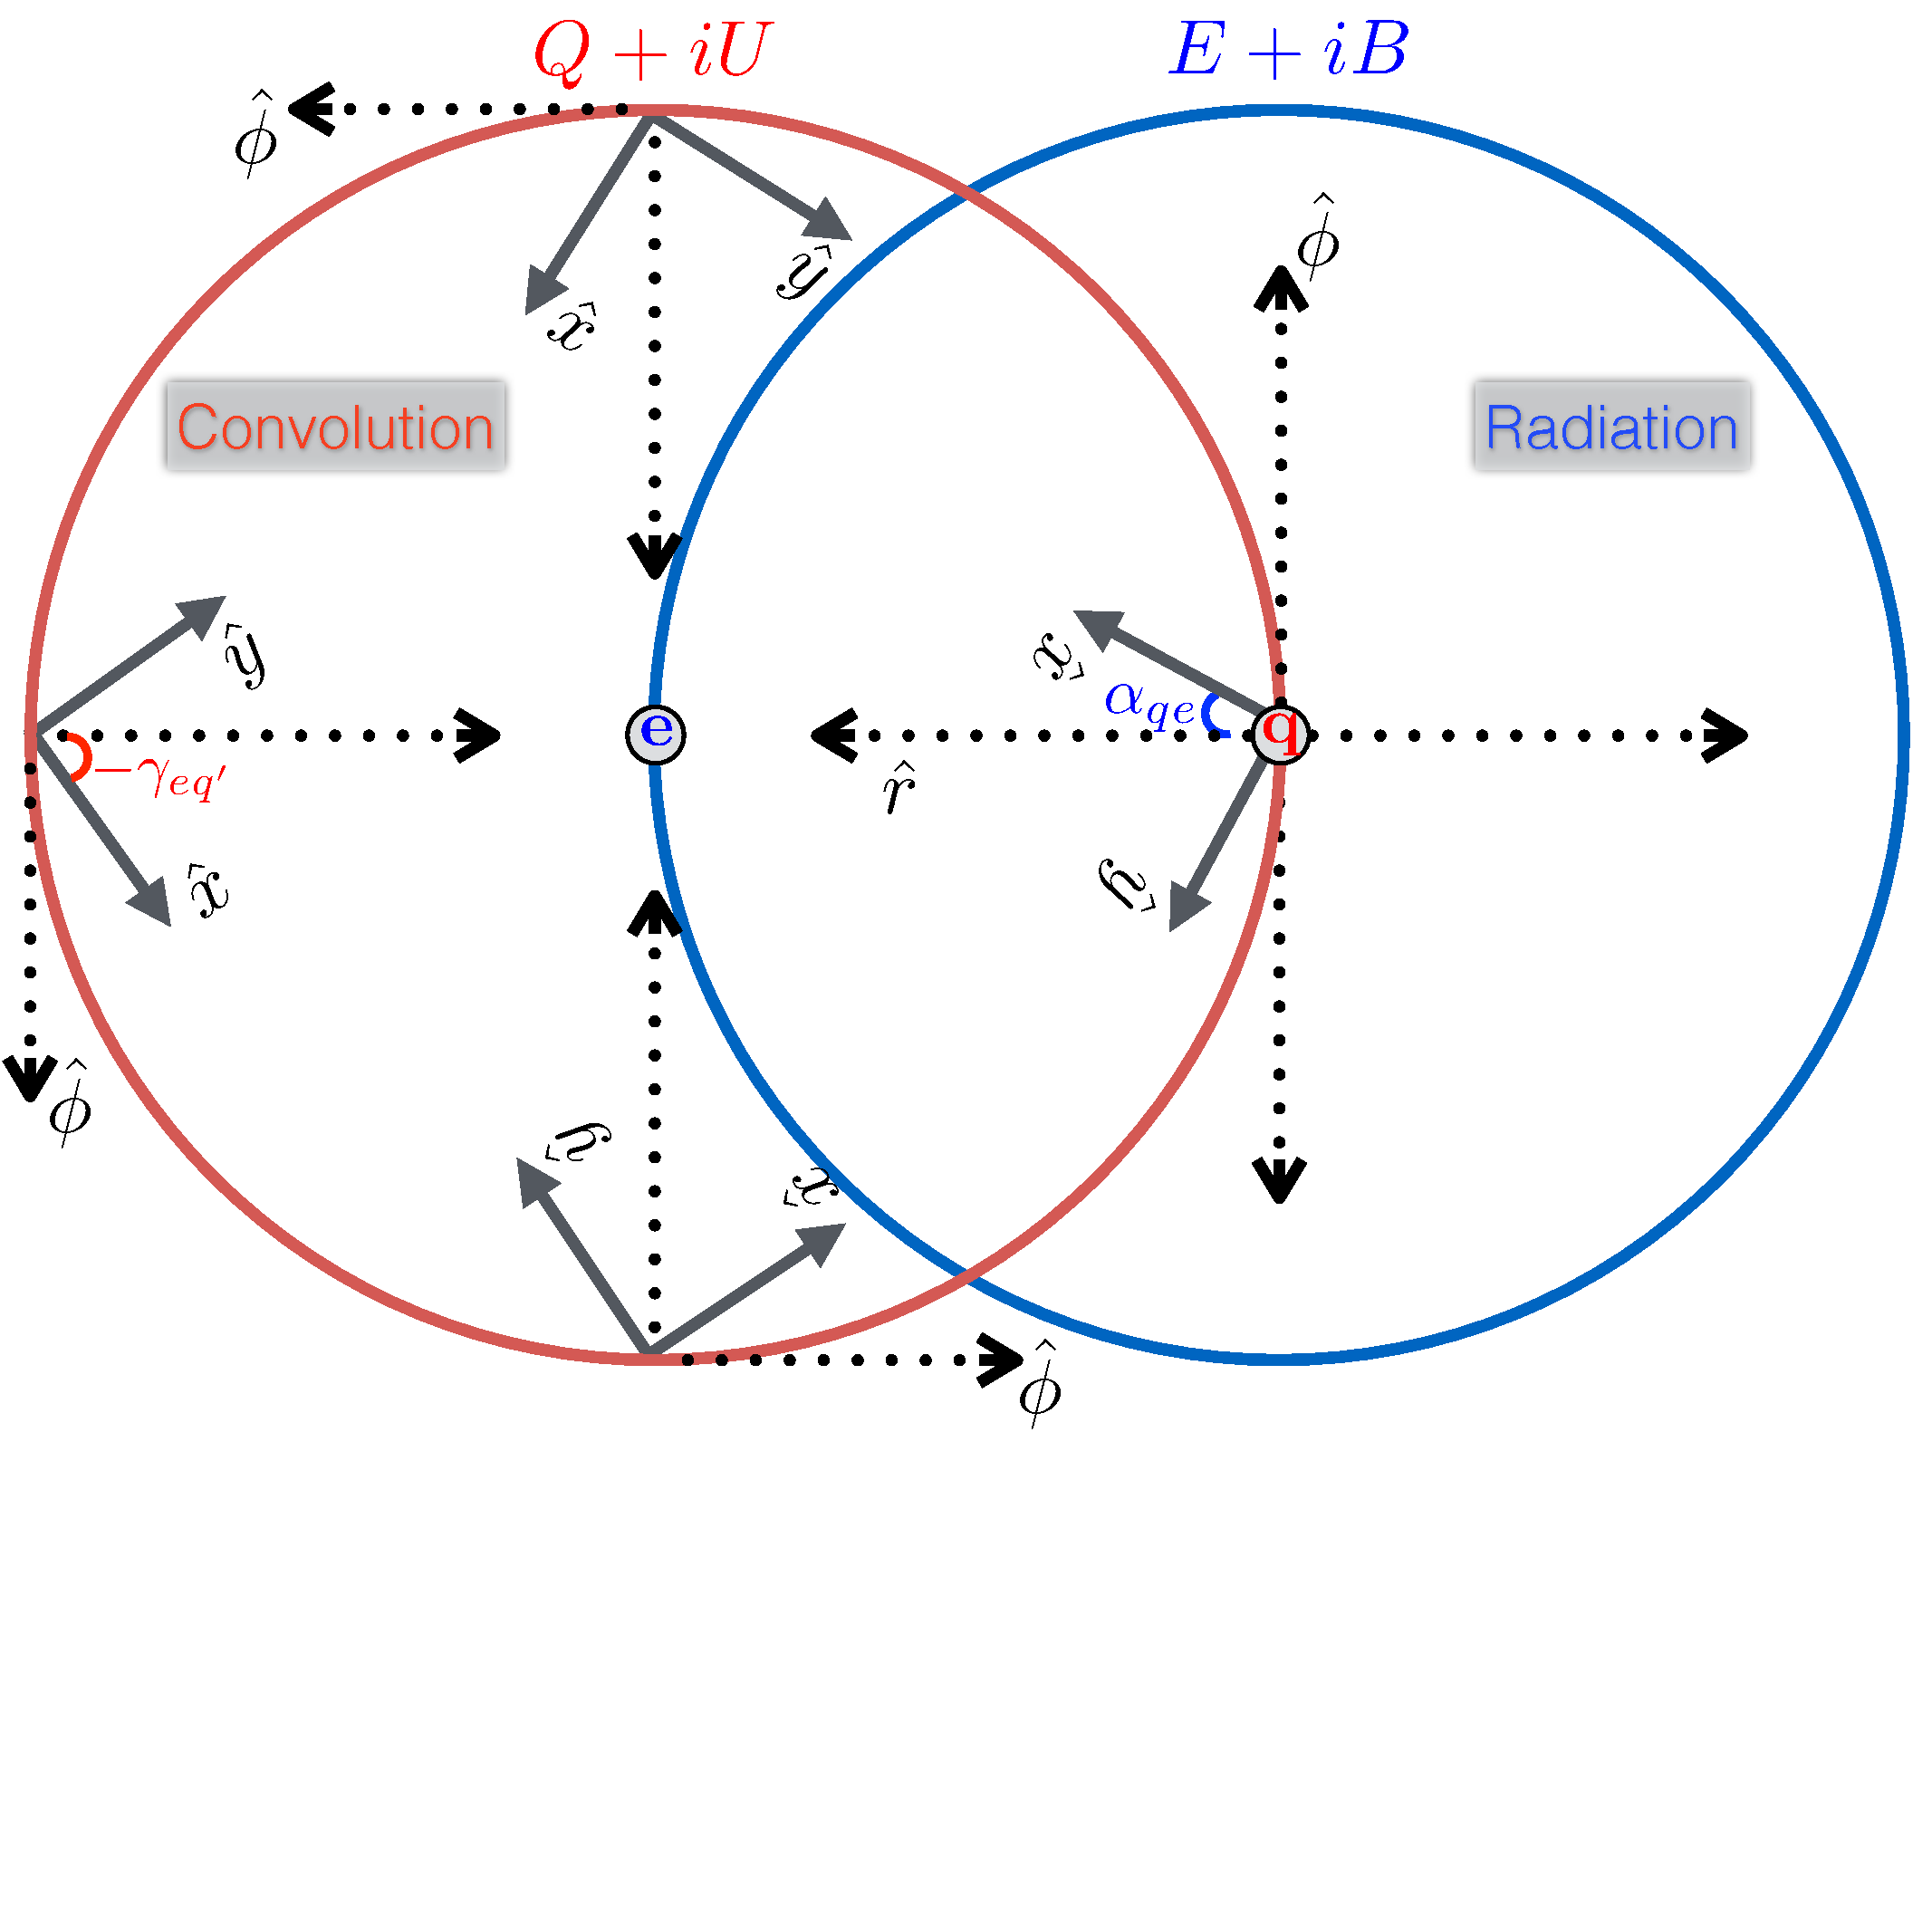
\includegraphics[width=0.5\columnwidth]{radiation_convolution.pdf}
\caption{The local cartesian coordinate are only drawn on the red circle, representative of the coordinate dependence of the Stokes parameters. The value of the scalar field at location `e' can be evaluated by summing over the contribution from all the Stokes parameters on the red circle (sphere). The convolutions are performed with kernels which are defined in term of the Euler angle $\gamma_{eq}$. Alternatively, one can compute the contribution from the Stokes parameter at location `q' to all the point on the blue circle(sphere) and this is a function of the Euler angle $\alpha_{eq}$. In the flat sky limit, since $\gamma=-\alpha$ there is no difference between the radiating and convolving kernels.}
\label{fig:planar_euler_angles}
\end{figure}
%

\textit{Convolution kernel:} We can also formulate the real space operator to be a function of Euler angles corresponding to the inverse rotation. The Euler angles for the inverse rotations (i.e. to align the coordinate system at $\hat{n}_e$ with that at $\hat{n}_q$) are related to the forward rotation Euler angles by the following relations: $\alpha_{eq}=-\gamma_{qe}$, $\beta_{eq} = -\beta_{qe}$ and  $\gamma_{eq} =-\alpha_{qe}$. Since the kernel only depends on the cosine of the Euler angle $\beta$, it is immune to changes in its sign. The operator equation can be expressed as a function of the Euler angle $\gamma_{eq}$ as follows, 
%
\beq \label{eq:qu2eb_convolution_explicit}
\bmat E_e \\ B_e  \emat =- \sum_{q=1}^{N_{\rm pix}}{{}_{\mm}f}(\beta_{eq},\ell_{\rm min},\ell_{\rm max})\bmat \cos(2 \gamma_{eq}) & -\sin(2\gamma_{eq})\\  \sin(2 \gamma_{eq})  & \cos(2 \gamma_{eq}) \emat  \bmat Q_q \\ U_q  \emat \Delta \Omega\,,
\eeq
%
%where $\Delta \Omega$ denotes the pixel area and all the symbols have their usual meaning. 
\revisit{This version of the real space operator would have naturally emerged had we simplified the the equivalent function $\sum_{\ell m} {}_{0}Y^*_{\ell m}(\hat{n}_e){}_{+2}Y_{\ell m}(\hat{n}_q)$ in \eq{eq:qu2eb_gen_kernel}.} This formulation of the real space operator can be interpreted as integrating at some fixed location $\hat{n}_e$ the $E/B$ mode contribution arising from the Stokes parameters at all location $\hat{n}_q$ on the sphere. This operation can be expressed more concisely as follows,
%
\begin{subequations} \label{q:qu2eb_convolution_concise}
\beqry 
[E + iB](\hat{n}_e) &=& - \Delta \Omega \sum_{q=1}^{N_{\rm pix}} \left(\sum_{\ell=\ell_{\rm min}}^{\ell_{\rm max}} \frac{2 \ell+1}{4 \pi} \sqrt{\frac{(\ell-2)!}{(\ell+2)!}} P_{\ell}^{2}(\beta_{eq}) \right) {\Bigg( e^{i2 \gamma_{eq}}   {}_{+2}X (\hat{n}_q) \Bigg)} \,, \label{eq:qu2eb_physical}\\
&=& \Bigg\lbrace \left[ - \Delta \Omega \sum_{\ell=\ell_{\rm min}}^{\ell_{\rm max}} \sqrt{\frac{2 \ell+1}{4 \pi}}Y_{\ell 2}(\beta_{eq},\gamma_{eq}) \right]  \circ {}_{+2}X \Bigg\rbrace(\hat{n}_e) \,, \\
&=& \Bigg\lbrace \mathcal{M}_{B} \circ {}_{+2}X \Bigg\rbrace(\hat{n}_e) \,, \label{eq:qu2eb_convolution} 
\eeqry
\end{subequations}
%
where $\circ$ denotes a convolution and $\mathcal{M}_{B}$ is merely the conjugated function $\mm^*$ when expressed as a function of the Euler angle $\gamma_{eq}$ it can be thought of as an effective instrument beam pointing to the direction $\hat{n}_e$. 
%--------------------------------------------------------


%--------------------------------------------------------
\subsection{Evaluating Stokes parameters $Q$ \& $U$ from scalar fields $E$ \& $B$}\label{sec:eb2qu}
The real space operator which translates $E$ \& $B$ fields to Stokes parameters $Q$ \& $U$ can be derived using a similar procedure. Expressed in the matrix-vector notation, inverse operator is given by,
%
\begin{subequations}
\beqry
\bar{P} &=& \bar{T}^{-1} *{{}_2\mathcal{Y}} *\tilde T *{{}_0\mathcal{Y}^{\dagger}}\bar{S} = \frac{1}{2} \bar{T}^{\dagger} *{{}_2\mathcal{Y}} *\tilde T *{{}_0\mathcal{Y}^{\dagger}}\bar{S} \,,  \\
&=&  \bar O^{-1} *\bar{S}\,.
\eeqry
\end{subequations}
%
%The inverse operator $\bar{O}^{-1}$ can be derived by realizing that $\mm^{-1}$ is given by the following expression,
%%
%\beq
%\mm^{-1} = \sum_{\ell m}  {{}_{2}}Y_{\ell m}(\hat n_q) {}_{0}Y^*_{\ell m}(\hat n_e) \, 
%\eeq
%%
The inverse operator expressed in terms of the function $\mm$ given in \eq{eq:qu2eb_gen_kernel} is given by the following equation,
%
\beq
{\bar O}^{-1}=-\bmat \mathcal{M}_{r} & -\mathcal{M}_{i} \\  \mathcal{M}_{i}  & \mathcal{M}_{r} \emat_{2 N_{\rm pix} \times 2 N_{pix}} =-{{}_{\mm}f}(\beta_{eq},\ell_{\rm min},\ell_{\rm max})\bmat \cos(2 \alpha_{qe}) & -\sin(2\alpha_{qe})\\  \sin(2 \alpha_{qe})  & \cos(2 \alpha_{qe}) \emat \,,
\eeq
%
where all the symbols have the same meaning as discussed in \sec{sec:qu2eb}. Note that the kernel in the above equation differs from the one in \eq{eq:op_qu2eb_rad} by a change in sign on the off-diagonals of the block matrix. When expressed in terms of the same set of Euler angles used to define the operator $\bar{O}$, it can be shown that the different forms of the real space operator are given by,
%
\beqry
{}_{+2}X(\hat{n}_q) &=& \Bigg\lbrace \mathcal{M}^*_{G} \circ [E+iB] \Bigg\rbrace(\hat{n}_q) \hspace{0.8cm} \textrm{\emph {Convolution kernel}}\,, \label{eq:eb2qu_convolution}\\
{}_{+2}X(\hat{n}_q) &=&  \sum_{e=1}^{N_{\rm pix}} [E+iB](\hat{n}_{e}) \cdot  \mathcal{M}^*_{B}[\hat{n}_e] \hspace{0.8cm} \textrm{\emph{Radiation kernel}}\,,
\eeqry
%
where all the symbols have the same meaning as defined in \sec{sec:qu2eb}. Note that the conjugated forms of the Green's function and the effective beam for the operator $\bar{O}$ have their roles reversed for the inverse operator $\bar{O}^{-1}$.
%--------------------------------------------------------


%--------------------------------------------------------
\subsection{Decomposing Stokes parameters $Q$ \& $U$  into those corresponding to $E$ \& $B$ modes respectively}
We can only measure the total Stokes vector which is a sum of the Stokes vectors corresponding to the respective scalar modes. The $E$ \& $B$ modes are orthogonal to each other, in the sense that their respective operators are orthogonal to each other as seen in \eq{eq:op_eb_ortho}. It is possible to decompose the Stokes vector \vp{} into one \vp{\rm E} that purely contributes to $E$ modes and another \vp{\rm B} that purely contribute to the $B$ modes of polarization. In this section we derive the real space operators which operate on the total Stokes vector and yield this decomposition, without ever having to explicitly evaluate the scalar modes. Though the algebra is a little more involved, the derivation is similar to that discussed in \sec{sec:qu2eb}, hence we refrain from presenting the detailed calculations here, but outline the key points. We use the harmonic space projection operators $\tilde O_{E/B}$, defined in \eq{eq:har_eb_op}, to derive the respective real space operators. The Stokes parameters corresponding to each scalar mode are given by the following expressions,
%
\beqry
\bar{P}_E &=&  [\bar T^{-1} * {{}_2\mathcal{Y}} *\tilde T * \tilde O_E* \tilde T^{-1}* {{}_2\mathcal{Y}^{\dagger}} *\bar T] *\bar{P}  \,, \\
&=& [\frac{1}{4} \bar T^{\dagger } * {{}_2\mathcal{Y}} *\tilde T * \tilde O_E* \tilde T^{\dagger} * {{}_2\mathcal{Y}^{\dagger}} *\bar T ]*\bar{P}  \,, \nonumber \\
&=&  \bar O_{E}*\bar{P} \,,\nonumber \\
\bar{P}_B &=&  [\bar T^{-1}* {{}_2\mathcal{Y}}* \tilde T* \tilde O_B* \tilde T^{-1}* {{}_2\mathcal{Y}^{\dagger}}* \bar T]*\bar{P}  \,, \\
&=& [\frac{1}{4} \bar T^{\dagger } * {{}_2\mathcal{Y}} *\tilde T * \tilde O_B* \tilde T^{\dagger} *{{}_2\mathcal{Y}^{\dagger}} *\bar T] *\bar{P}   \,, \nonumber\\
&=&  \bar O_{B}*\bar{P} \,. \nonumber
\eeqry
%
We contract over all the matrix operators to arrive at the the real space operators. On working through the algebra it can be shown that the real space operators have the following form,
%
\beq
\bar O_{E/B} = 0.5 \bmat \mathcal{I}_{r} & \mathcal{I}_{i} \\  -\mathcal{I}_{i}  & \mathcal{I}_{r} \emat \pm 0.5 \bmat \mathcal{D}_{r} & \mathcal{D}_{i} \\  \mathcal{D}_{i}  & - \mathcal{D}_{r} \emat \,,\\
\eeq
where $\mathcal{I}_{r} ~\&~ \mathcal{D}_{r}$ and $\mathcal{I}_{i} ~\&~ \mathcal{D}_{i}$ are the real and complex parts of the following complex functions,
%
\begin{subequations}
\beqry
\mathcal{I} (\hat{n}_e,\hat{n}_q) &=& \mathcal{I}_{r} + i \mathcal{I}_{i} = \sum_{\ell m} {_{-2}Y}_{\ell m}(\hat n_e) {_{-2}Y}^*_{\ell m}(\hat n_q) \,, \\
\mathcal{D}(\hat{n}_e,\hat{n}_q)  &=& \mathcal{D}_{r} + i\mathcal{D}_{i} = \sum_{\ell m} {_2Y}_{\ell m}(\hat n_e) {_{-2}Y}^*_{\ell m}(\hat n_q) \,.
\eeqry
\end{subequations}
%
These functions can be further simplified using the identity of spin spherical harmonics given in \eq{eq:sum_spin_shf}. Specifically it can be shown that these functions reduce to the following mathematical forms,
%
\beqrys \label{eq:fn_i}
\mathcal{I}(\hat{n}_e, \hat{n}_q) &=& \sum_{\ell} \sqrt{\frac{2\ell+1}{ 4 \pi}}{_{-2}Y}_{\ell2}(\beta_{qe}, \alpha_{qe}) ~ \rm{e}^{i2 \gamma_{qe}} \label{eq:healpix-compatible-i} = \mathcal{I}_r + i \mathcal{I}_i \,, \\
\mathcal{I}_r + i \mathcal{I}_i &=& \Big [ \cos(2 \alpha_{qe} +  2\gamma_{qe}) + i \sin(2 \alpha_{qe} +  2 \gamma_{qe}) \Big]   {{}_{\mi}f}(\beta_{qe},\ell_{\rm min},\ell_{\rm max}) \,,
\eeqrys
%
%
\beqrys \label{eq:fn_d}
\mathcal{D}(\hat{n}_q, \hat{n}_e) &=& \sum_{\ell} \sqrt{\frac{2\ell+1}{ 4 \pi}}{_2Y}_{\ell 2}(\beta_{qe}, \alpha_{qe}) ~ \rm{e}^{- i2 \gamma_{qe}} \label{eq:healpix-compatible-m} =\mathcal{D}_r + i \mathcal{D}_i \,, \\
\mathcal{D}_r + i \mathcal{D}_i &=&  \Big [ \cos(2 \alpha_{qe} - 2\gamma_{qe}) + i \sin(2 \alpha_{qe} -  2 \gamma_{qe}) \Big]   {{}_{\md}f}(\beta_{qe},\ell_{\rm min},\ell_{\rm max}) \,,
\eeqrys
%
where the radial functions are given by,
%
\beq
{{}_{\mdi}f}(\beta,\ell_{\rm min},\ell_{\rm max}) = \sum_{\ell=\ell_{\rm min}}^{\ell_{\rm max}} \sqrt{\frac{2\ell+1}{ 4 \pi}} {{}_{ \mdi}f}_{\ell}(\beta) \label{eq:f2_rad_ker}\,,
\eeq
%
where the functions ${{}_{ \pm 2}f}_{\ell}(\beta)$ are expressed in terms of $P_{\ell}^2$ Legendre polynomials and are given by the following explicit mathematical forms,
 %
 \beqry
 _{\mdi}f_{\ell}(\beta) &=& 2 \frac{(\ell-2)!}{(\ell+2)!}  \sqrt{\frac{2\ell +1 }{4 \pi}} \Bigg[ - P_{\ell}^{2} (\cos  \beta) \left( \frac{\ell-4}{\sin^2 \beta} + \frac{1}{2}\ell(\ell-1) \pm \frac{2 (\ell-1) \cos \beta}{\sin^2 \beta} \right) \nonumber \\ 
&+& P_{\ell-1}^2 (\cos \beta) \left( (\ell+2) \frac{\cos \beta}{\sin^2 \beta} \pm \frac{2 (\ell+2)}{ \sin^2 \beta } \right) \Bigg] \,. \label{eq:rad_ker_quequbqu}
 \eeqry
 %
Finally the Stokes parameters corresponding to the respective scalar fields can be computed by evaluating the following expressions, 
 %
\beqry \label{eq:op_qu2equbqu}
\bmat Q_e \\ U_e  \emat_{E/B} &=& \sum_{q=1}^{N_{\rm pix}} \Bigg\lbrace {{}_{\mi}f}(\beta_{qe},\ell_{\rm min},\ell_{\rm max}) \bmat \cos(2 \alpha_{qe} + 2\gamma_{qe}) & \sin(2\alpha_{qe} +2 \gamma_{qe}) \\  -\sin(2\alpha_{qe} +2 \gamma_{qe})  & \cos(2 \alpha_{qe} + 2 \gamma_{qe}) \emat  \bmat Q_q \\ U_q  \emat  \\ &\pm& {}_{\md}f(\beta_{qe},\ell_{\rm min},\ell_{\rm max}) \bmat \cos(2 \alpha_{qe} - 2\gamma_{qe}) &  \sin(2\alpha_{qe} - 2 \gamma_{qe}) \\  \sin(2\alpha_{qe} - 2 \gamma_{qe})  & - \cos(2 \alpha_{qe} - 2 \gamma_{qe}) \emat  \bmat Q_q \\ U_q  \emat \Bigg\rbrace 0.5 \Delta\Omega  \,, \nonumber 
\eeqry
%
where all the symbols have their usual meaning. The above expression can be cast in the further simplified form,
%
\beqry
{}_{+2}X_{E/B}(\hat{n}_e) &=&0.5 \Delta \Omega\sum_{q=1}^{N_{\rm pix}}  {{}_{\mi}f}(\beta_{qe}) e^{-i2 (\alpha_{qe} + \gamma_{qe})} {}_{+2}X(\hat{n}_q) \pm {{}_{\md}f}(\beta_{qe}) e^{i2 (\alpha_{qe} - \gamma_{qe})} {}_{+2}X(\hat{n}_q)^* \,, \nonumber \\
&=& 0.5 \Bigg\lbrace \mathcal{I}^* \circ {}_{+2}X\pm \mathcal{D} \circ {}_{+2}X^* \Bigg\rbrace \,, \label{eq:qu2equbqu_convolution}
\eeqry
%
where we have suppressed the explicit multipole dependence of functions ${}_{\mdi}f$ for brevity. \revisit{Comment on the radiating and convolution form of the operators.}

\comment{Recheck the math described below}
The operator $\mathcal{I}$ is a band limited version of the delta function ($\lim_{\ell \rightarrow \infty} \mathcal{I} = \delta(\hat{n}_i - \hat{n}_j)$) for spin-2 fields. When interpreted as a matrix it is a band limited version of the identity matrix. Though it has non-vanishing off diagonal elements ($\mathcal{I} \neq 0 $ when $\hat{n}_i \neq \hat{n}_j$) owing to the band limit, for all practical purposes $\mathcal{I}$ acts like an identity operator as is confirmed by the following set of identities: (i) $\mathcal{I}*\mathcal{I}=\mathcal{I}$ ; (ii) $\mathcal{D}*\mathcal{I}=\mathcal{D}$. Also $\mathcal{D}^*$ is the inverse of $\mathcal{D}$ in this band limited sense: $\mathcal{D}^**\mathcal{D}=\mathcal{I}$. It is useful to note that the operator $\mathcal{D}$ is a complex but symmetric matrix and $\mathcal{I}$ is an Hermitian operator. Using these properties of the operators $\mathcal{I}$ and $\mathcal{D}$, one can verify that the real space operators satisfy the following identities,
%
\begin{subequations}
\beqry
\bar O_E * \bar O_E &=& \bar O_E ~~;~~ \bar O_B * \bar O_B = \bar O_B \,, \\
\bar O_E*\bar O_B &=& 0 \,,\\
\bar O_E + \bar O_B &=& \mathcal{I} \,,
\eeqry
\end{subequations}
%
which are the real space analogues of \eq{eq:har_op_prop}. While testing the above stated identities one encounters terms like $\mathcal{D}*\mathcal{I}^*,\mathcal{I}^**\mathcal{I} \textrm{ and }  \mathcal{I}*\mathcal{I}^*$ which cannot be simply interpreted, but they always occur in pairs with opposite signs, hence exactly cancel each other. 

Note that unlike in the harmonic case, the sum of the operators is not exactly an identity matrix. 
%\comment{Isn't it possible to do some real space operations which doesn't care for the band limit but still returns the required decomposition into the respective scalar modes ?} 
This non-exactness is representative of the loss of information resulting from making this transformation on the measured data with some imposed band limit. Forcing the sum of the operators to be exactly an identity matrix compromises the orthogonality property of the $\bar{O}_E$ \& $\bar{O}_B$ operators, which is exact.